\newpage
\section {Билет 4. Индексы (дерево, карты, хэш).}

Индекс применяется для ускорения поиска нужных строк (в операциях
выборки, обновления и удаления). Индекс является упорядоченной структурой (записи в индексе хранятся в отсортированном виде). После создания индекса в актуальном состояние его поддерживает СУБД.

По умолчанию команда CREATE INDEX создаёт индексы на основе B-деревьев, эффективные в большинстве случаев (в дальнейшем такие индексы будем называть индекс-В-дерево). Выбрать другой тип можно, написав название типа индекса после ключевого слова USING.

\textbf{B-дерева:} 

Структура B-дерева: 
\begin{itemize}
    \item При построении B-дерева применяется фактор t, который называется минимальной степенью. Каждый узел, кроме корневого, должен иметь, как минимум t – 1, и не более 2t – 1 ключей. Обозначается n[x] – количество ключей в узле x.
    \item Ключи в узле хранятся в неубывающем порядке. Если x не является листом, то он имеет n[x] + 1 детей. Если занумеровать ключи в узле x как k[i], а детей c[i], то для любого ключа в поддереве с корнем c[i] (пусть k1), выполняется следующее неравенство $-k[i-1] \leq k1 \leq k[i]$ (для $c[0]: k[i-1] = -\infty,$ а для $c[n[x]]: k[i] = +\infty)$. Таким образом, ключи узла задают диапазон для ключей их детей.
    \item Все листья B-дерева должны быть расположены на одной высоте, которая и является высотой дерева. Высота B-дерева с $n \geq 1$ узлами и минимальной степенью $t\geq 2$ не превышает logt(n+1).
\end{itemize}

На рисунке \ref{fig:tree} изображен пример B-дерева. 

\begin{figure}[!h]
    \centering
    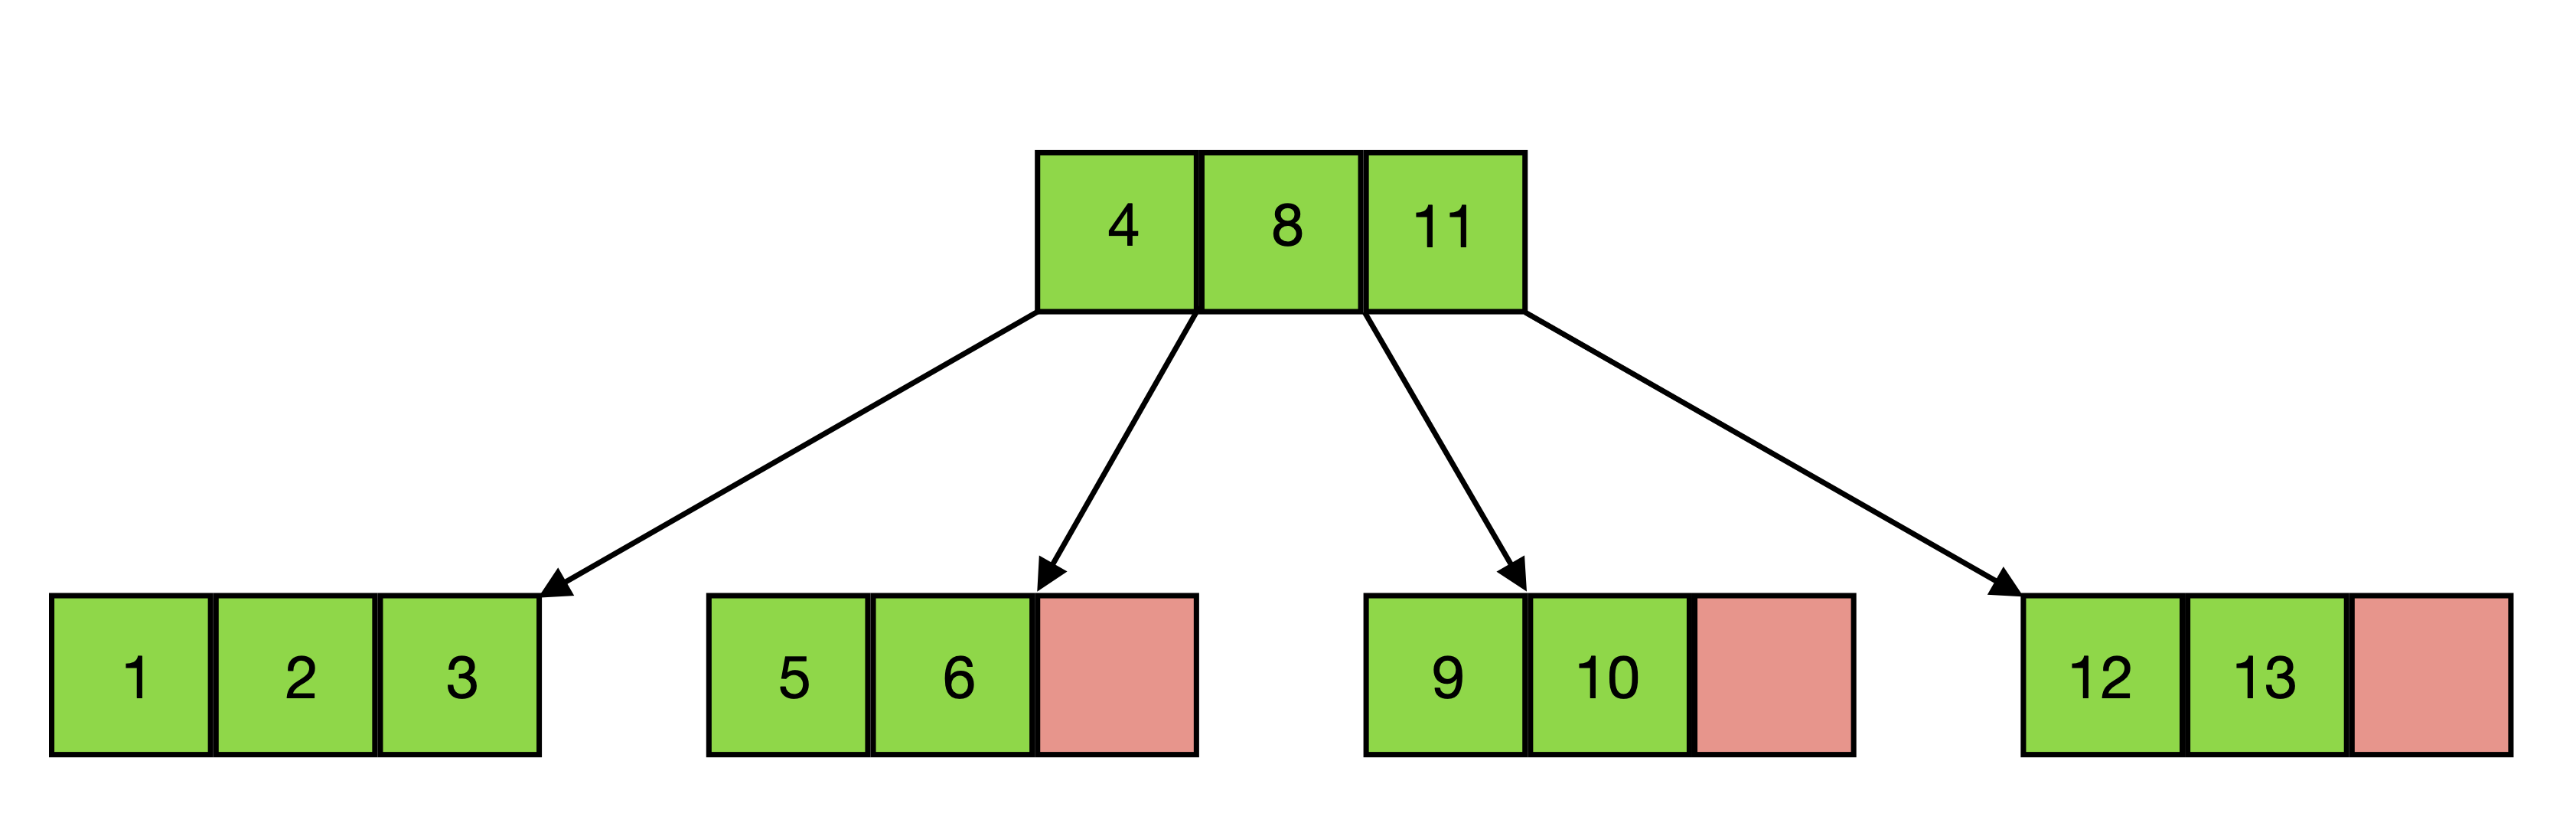
\includegraphics[scale = 0.1]{4/B-tree.png}
    \caption{Пример B-дерева}
    \label{fig:tree}
\end{figure}


B-деревья могут работать в условиях на равенство и в проверках диапазонов с данными, которые можно отсортировать в некотором порядке. Точнее, планировщик запросов PostgreSQL может задействовать индекс-B-дерево, когда индексируемый столбец участвует в сравнении 

\textit{Недостатки}: поиск только по одному столбцу. Например, если нам нужно найти брюнетов с зелеными глазами, то по дереву мы найдем брюнетов, а дальше уже придется проверять их всех, то есть не использовать индексы. 

\textbf{Bitmap(карты)} 

В bitmap-структурах создается двухмерный массив со столбцом для каждой строки в индексируемой таблице. Каждый столбец представляет отдельное значение в bitmap-индексе. Этот двухмерный массив показывает каждое значение индекса, умноженное на количество строк в этой таблице.

Идея поиска по такому индексу предсавленна на рисунке \ref{fig:Map}  

\begin{figure}[!h]
    \centering
    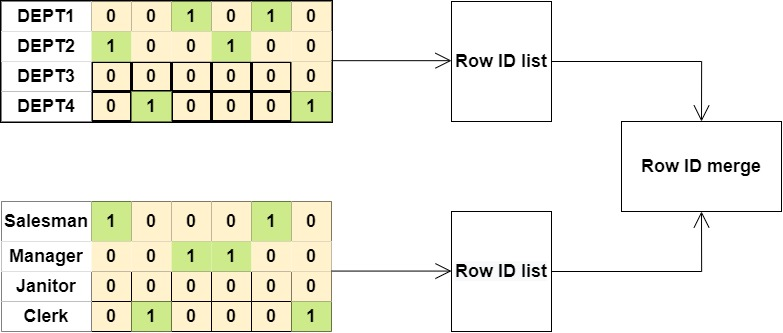
\includegraphics[scale = 0.5]{4/Index.jpg}
    \caption{Пример поиска по индексу}
    \label{fig:Map}
\end{figure}


Берем строчку из первого индекса (по нашим условиям), и строчку из второго индекса. Дальше логические операции заменяем на побитовые и проводим их на наших выбранных строчках (Рис.\ref{fig:BMap}).

\begin{figure}[!h]
    \centering
    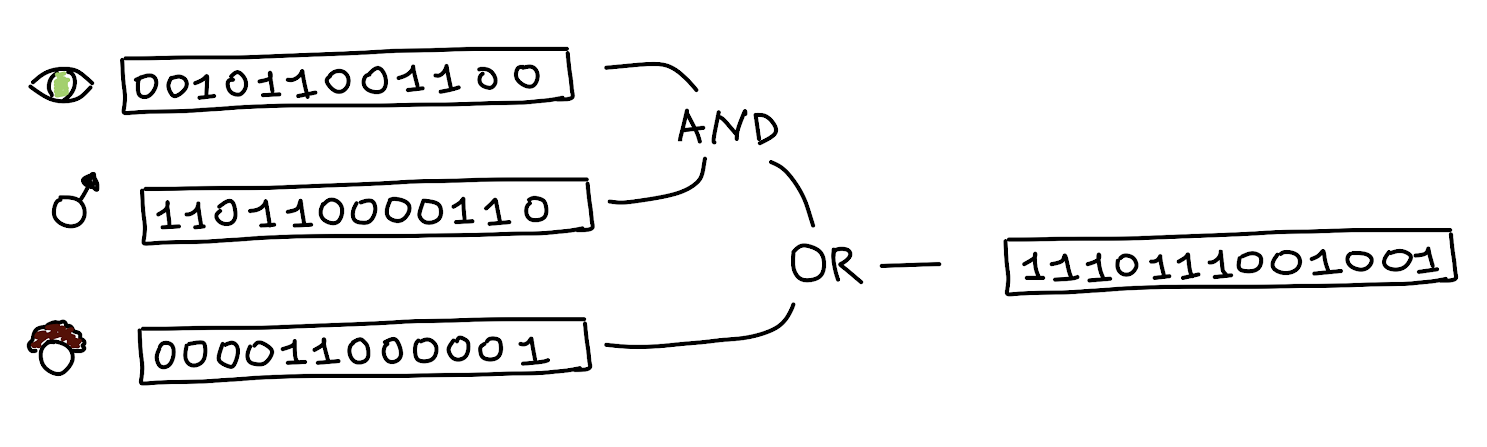
\includegraphics[scale = 0.4]{4/BitMat.png}
    \caption{Пример поиска по индексу}
    \label{fig:BMap}
\end{figure}

\textit{Недостатки:} предположим, мы заблокировали запись -> нужно заблокировать часть индекса, где она учавствует (в дереве - только лист, там мало значений: k), а вот у карты нужно блокировать всю строку индекса - это много.


\textbf{Хеш - индексы} 

Хэш-индекс (Hash Index) основан на хэш-таблице, он полезен только для точного поиска по каждому столбцу в индексе. Просто по значениям в таблице вычисляем некоторую хеш-функцию и значения таблицы помещаем в ячейку с номером хеша. 

